\documentclass[conference]{IEEEtran}

\usepackage{cite}
\usepackage{amsmath,amssymb,amsfonts}
\usepackage{graphicx}
\usepackage{textcomp}
\usepackage{xcolor}
\usepackage{booktabs}
\usepackage{array}
\usepackage{url}

\graphicspath{{figures/}}
% run in heading used inside sections to save space
\newcommand{\runin}[1]{\par\noindent\textit{#1}\ }

\begin{document}

\title{AsiaCupT20: A Dataset of the 2022 and 2025 Asia Cup Cricket Tournaments with Scorecard, Pitch and Weather Information}

\author{
\IEEEauthorblockN{Author One}
\IEEEauthorblockA{\textit{Department of [Department]} \\
\textit{[University]}\\
Dhaka, Bangladesh \\
email1@example.com}
\and
\IEEEauthorblockN{Author Two}
\IEEEauthorblockA{\textit{Department of [Department]} \\
\textit{[University]}\\
Dhaka, Bangladesh \\
email2@example.com}
\and
\IEEEauthorblockN{Author Three}
\IEEEauthorblockA{\textit{Department of [Department]} \\
\textit{[University]}\\
Dhaka, Bangladesh \\
email3@example.com}
}

\maketitle

\begin{abstract}
Cricket followers often ask simple questions, such as whether it is better to bat second and whether the toss matters. To answer them, researchers need clean match records, but the records of recent Asia Cup tournaments are spread over many web pages and are often incomplete. This paper describes AsiaCupT20, a dataset of all 32 matches of the 2022 and 2025 Asia Cup T20 tournaments, which were both played in the United Arab Emirates. We compiled the 2022 matches ourselves and extended an openly licensed table of the 2025 matches. Each match has 58 fields, including teams, toss, scores, powerplay runs, extras, result, officials, ground size, and short notes on the pitch and weather with their sources. A second table gives playing elevens and batting and bowling figures for 2025. We corrected errors in the source records, added calculated fields, and ran 13 automatic checks, which all passed. In a first example of use, chasing teams won 19 of 31 completed matches, but this small sample cannot rule out chance. The dataset and code are shared for reuse.

\end{abstract}

\begin{IEEEkeywords}
cricket, Asia Cup, T20 international, open dataset, sports analytics, pitch and weather, data quality
\end{IEEEkeywords}

\section{Introduction}
Cricket matches produce a lot of numbers. Each ball is recorded, and every match ends with a full account of who batted, who bowled and who won. Fans use these records to argue about their teams, coaches use them to decide whether to bat or bowl after winning the toss, and researchers use them to study how the game works.

These records are not always easy to use. Web scorecards are made for reading, so the same facts appear on several pages, often spelled in different ways. Notes on the pitch and the weather usually sit in news previews and not in a table beside the scores. Raza and Ali recently released a match level table for the 2025 Asia Cup \cite{razaarxiv,razadata}, and we build on it in this paper. We did not find one table that covers both the 2022 and the 2025 tournaments and also records notes on the pitch and the weather.

AsiaCupT20 joins the two tournaments in one table with the same fields for every match. It adds pitch and weather notes with their sources, calculated fields, and a detailed scorecard sheet for 2025. We fixed errors found in the source records and tested the result with 13 automatic checks. We also give a short first analysis to show how the data can be used. The Asia Cup matters to readers in Bangladesh and across South Asia, and we hope a clean record helps students and young researchers ask real questions without first spending weeks copying numbers.

Section~\ref{sec:related} reviews related work and Section~\ref{sec:collection} explains how the data were built. Section~\ref{sec:description} describes the contents and Section~\ref{sec:validation} reports the checks. Section~\ref{sec:analysis} shows example uses, and Section~\ref{sec:limits} gives limits and usage notes. Table~\ref{tab:glossary} explains the main terms in plain words.

\begin{table}[!t]
\caption{Terms used in this paper, in plain words}
\label{tab:glossary}
\centering
\footnotesize
\renewcommand{\arraystretch}{1.08}
\begin{tabular}{@{}p{0.27\columnwidth}p{0.67\columnwidth}@{}}
\toprule
\textbf{Term} & \textbf{Meaning} \\
\midrule
Batting first, chasing & The side batting first sets a total. The chasing side must beat it. \\
Powerplay & The first six overs, when only a few fielders may stand far from the bat. \\
Extras & Runs given away without the batter hitting the ball, such as wides. \\
Super Over & A one over contest that settles a match ending level. \\
Elo rating & A strength score that rises after a win and falls after a loss, like a chess rating. \\
Range & Values likely to contain the true figure. A wide range means less certainty. \\
\bottomrule
\end{tabular}
\end{table}


\section{Related Work}
\label{sec:related}
Most earlier studies of cricket results try to predict the winner. Bailey and Clarke predicted one day international results while the game was in progress \cite{bailey2006}, and Asif and McHale later used a model whose settings change smoothly as the match goes on \cite{asif2016}. Morley and Thomas studied home advantage and other factors in English one day matches \cite{morley2005}. Kapadia et al.\ tested several methods on Indian Premier League data and found that none predicted well when only toss information was used \cite{kapadia2022}. Shah et al.\ compared seven methods on 458 T20 internationals to predict the result of high run chases \cite{shah2025}, and Suseela et al.\ compared four common classifiers \cite{suseela2025}. Many of these studies give one accuracy figure from a small sample, which can look better or worse than the truth.

On the data side, Cricsheet offers ball by ball records for many matches \cite{cricsheet}. For the 2025 Asia Cup, Raza and Ali released a match level dataset with 61 variables and a first look at the toss, team scores and boundaries \cite{razaarxiv,razadata}. Our work extends that effort in three ways. It covers two tournaments instead of one. It adds notes on the pitch and the weather with their sources. It also comes with automatic checks and a worked example of analysis.

\section{Data Collection and Cleaning}
\label{sec:collection}
\begin{figure*}[!t]
\centering
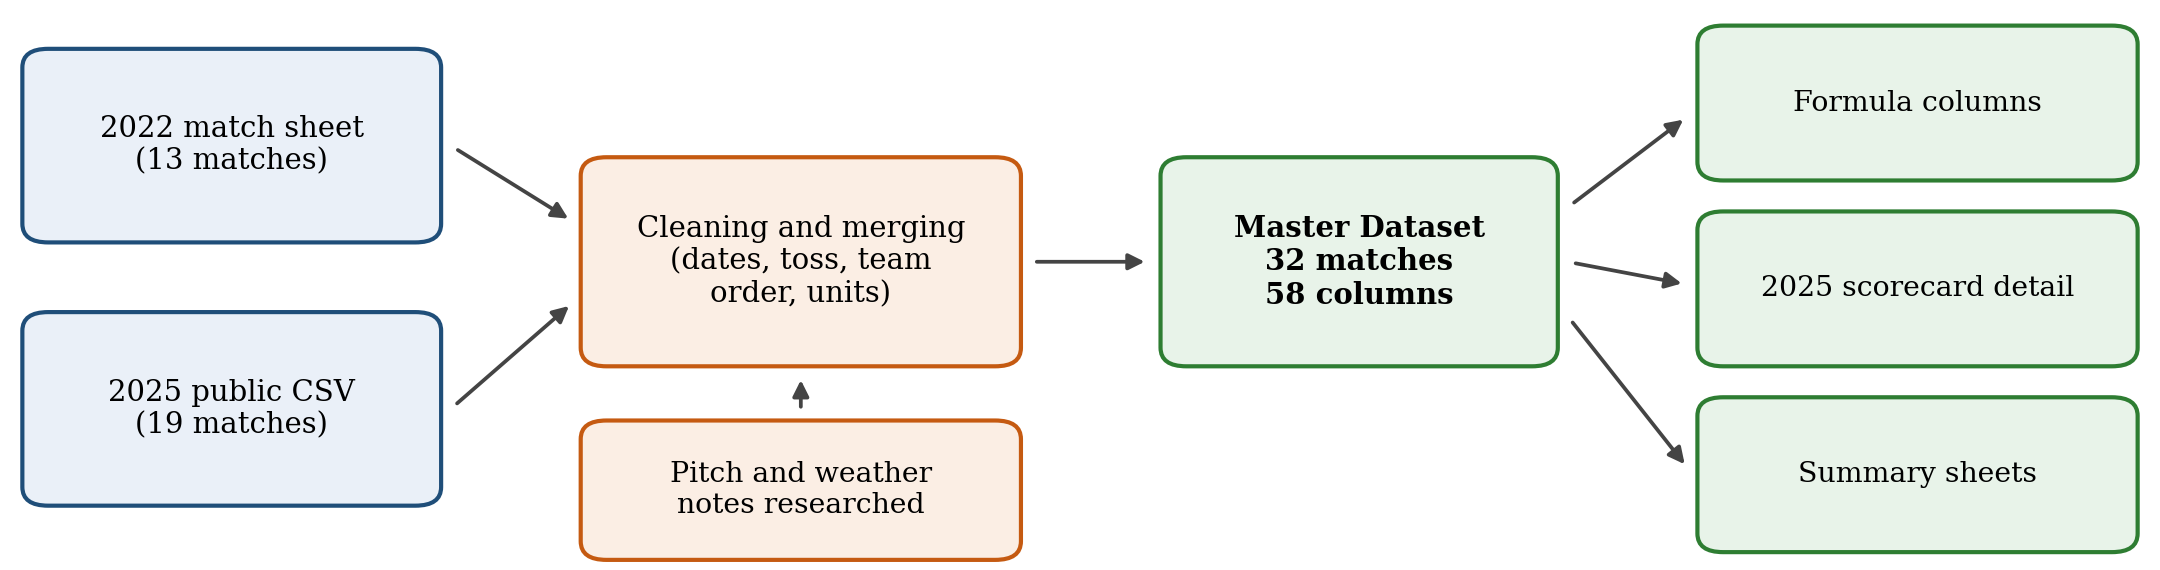
\includegraphics[width=0.9\textwidth]{fig_pipeline.png}
\caption{How the dataset was built. Two source files were cleaned and merged into one master table, extended with researched pitch and weather notes, and used to produce calculated fields, a detailed 2025 sheet and summary sheets.}
\label{fig:pipeline}
\end{figure*}

\runin{Scope.} Both tournaments were played in the T20 international format in the UAE. The 2022 edition had six teams and 13 matches, played at Dubai and Sharjah. The 2025 edition had eight teams, adding Oman and the UAE, and 19 matches, played at Dubai and Abu Dhabi. Each began with a group stage, followed by a Super Four stage and a final. Over the two years there were 18 group matches, 12 Super Four matches and 2 finals. Sri Lanka won in 2022 and India won in 2025.

\runin{Sources.} The 2022 rows were compiled by the authors, one row for each match. For 2025 we started from the dataset of Raza and Ali \cite{razadata}, which is shared under the CC BY 4.0 licence. Its authors collected the scorecards from ESPNcricinfo and checked them against information from the Asian Cricket Council \cite{razaarxiv,espn,acc}. We kept their match records, changed the layout, and made the corrections listed below. As the licence asks, we credit the original authors and state our changes.

For the 2025 pitch and weather notes we searched match by match. The weather condition came from the match page of a cricket website when one was available \cite{wisden}. Temperature, humidity and wind came from forecasts quoted in news previews, and the pitch descriptions came from previews, toss reports and expert reports \cite{news}. Each note carries a short text that names its source. We followed one rule, which was not to guess. For 2025, pitch notes exist for all 19 matches, weather condition for 17, temperature for 6, humidity for 2 and wind speed for 2. The temperature, humidity and wind figures are forecasts and not readings.

\runin{Errors fixed.} Joining sources turned up some small errors. Nine dates in the 2022 rows had the day and month swapped, so that 1 September appeared as 9 January. We rebuilt them and checked each one against the day of the week. The toss winner of India against Pakistan on 28 August 2022 was recorded as Pakistan, but match reports show that India won the toss and chose to field. In the 2025 file the first team column follows the schedule and not the batting order, so we reordered it. In our table \emph{Team~1 is always the side that batted first}. The 2025 file gave one start time for every match, but the organisers set most matches for 6:30 pm UAE time and one for 4 pm \cite{news}. We wrote the correct times together with Bangladesh time. We also replaced the title row with a plain header and used one spelling for each team and venue.

\runin{Fields added.} We added a match ID, series, stage, city and format, and 15 calculated fields written as spreadsheet formulas, so anyone can see how each value is worked out. One 2025 match, India against Sri Lanka in the Super Four stage, finished level at 202 runs each and was settled by a Super Over. We kept it and marked it clearly, so users can leave it out of win and loss analysis.

\section{Dataset Description}
\label{sec:description}
The dataset is one workbook with seven sheets. The \emph{Master Dataset} has one row per match, so 32 rows and 58 columns. The \emph{2025 Scorecard Detail} sheet has 19 rows and 53 columns. For each side it lists the playing eleven, the coach, the batting and bowling figures, the fall of wickets, the extras split into byes, leg byes, wides and no balls, and the fours and sixes. We added boundary runs and run rate to this sheet. Team Records, Tournament Summary, Venue Analysis and Player of the Match are summaries that recalculate from the master table, and a README sheet lists notes and known gaps.

Table~\ref{tab:fields} groups the 58 fields. \emph{Team~1 always means the side that batted first.} Dates are real dates, lengths are in metres and wind speed is in kilometres per hour. Table~\ref{tab:summary} gives a picture of the two tournaments. Of the 32 matches, 20 were played at Dubai, 8 at Abu Dhabi and 4 at Sharjah, and only Dubai hosted matches in both years.

\begin{table}[!t]
\caption{Summary of the two tournaments}
\label{tab:summary}
\centering
\footnotesize
\begin{tabular}{@{}lcc@{}}
\toprule
 & \textbf{2022} & \textbf{2025} \\
\midrule
Teams and matches & 6 and 13 & 8 and 19 \\
Champion & Sri Lanka & India \\
Runner up & Pakistan & Pakistan \\
Average runs per match & 301.2 & 289.8 \\
Highest and lowest team score & 212 and 38 & 202 and 57 \\
Won by chasing and batting first side & 9 and 4 & 10 and 8 \\
Decided by Super Over & 0 & 1 \\
\bottomrule
\end{tabular}
\end{table}


Figure~\ref{fig:completeness} shows how complete each group of fields is. Identity, teams, scores, results and pitch notes are complete for both years. Weather is complete for 2022 but only about 2842\% filled for 2025. The Abu Dhabi boundary lengths and the 2025 reserve umpire are missing. We leave these gaps visible because an empty cell is easier to handle than a number that was made up.

\begin{figure}[!t]
\centering
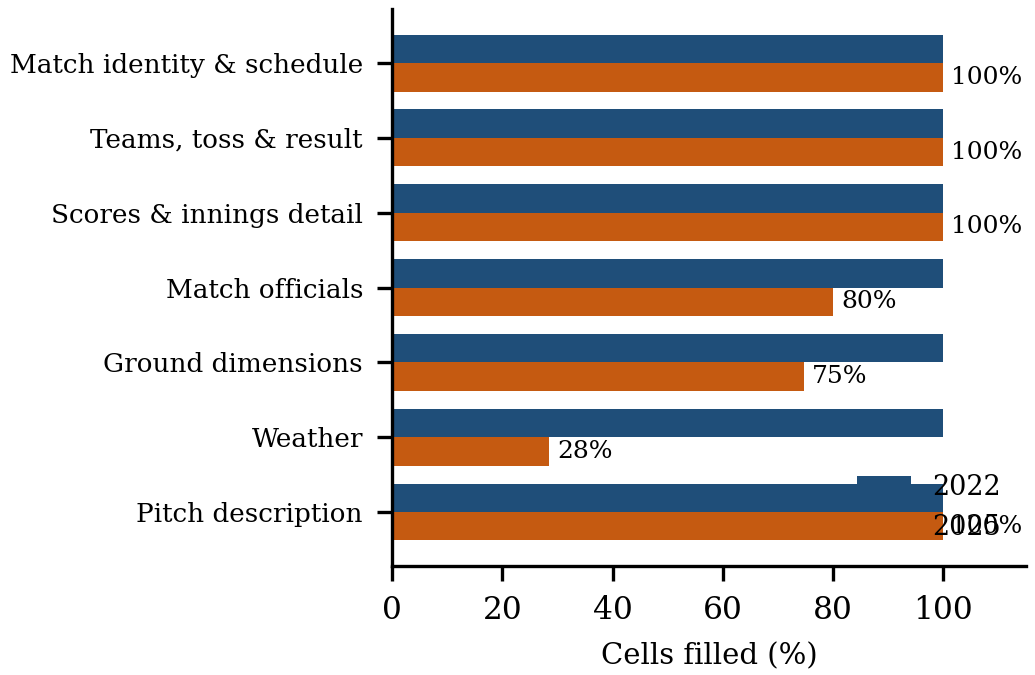
\includegraphics[width=\columnwidth]{fig_completeness.png}
\caption{Share of cells filled in, by group of fields. Numbers beside the orange bars are for 2025. Every 2022 group is complete.}
\label{fig:completeness}
\end{figure}

\begin{table*}[!t]
\caption{The 58 fields of the Master Dataset, grouped by purpose}
\label{tab:fields}
\centering
\footnotesize
\renewcommand{\arraystretch}{1.08}
\begin{tabular}{@{}p{0.14\textwidth}c p{0.48\textwidth}p{0.27\textwidth}@{}}
\toprule
\textbf{Group} & \textbf{No.} & \textbf{Fields} & \textbf{What they tell us} \\
\midrule
Identity and schedule & 13 & Match ID, Series, Year, Match Number, Match Label, Date, Group, Stage, Day, Time, Format, Venue, City & Which match, when and where \\
Ground size & 5 & Straight, Square and Mid Wicket Boundary Length, Wicket-to-Wicket Length, Pitch Width & Size of the playing area in metres \\
Weather and pitch & 7 & Temperature, Humidity, Condition, Wind Speed, Wind Direction, Pitch Condition, Weather \& Pitch Source & Conditions and where each note came from \\
Teams, toss, result & 7 & Team 1, Team 2, Toss Winner, Elected First, Match Winner, Player of The Match, Won by & Who played, the toss choice, who won and by how much \\
Scores & 6 & Team 1 Run, Team 2 Run, Powerplay Run Team 1 and 2, Team 1 and 2 Extras & Runs, first six overs, extras \\
Officials & 5 & Umpire 1, Umpire 2, TV Umpire, Reserved Umpire, Match Referee & Who ran the match \\
Calculated & 15 & Batting First, Batting Second, 1st and 2nd Innings Score, Match Loser, Result Type, Winner Batted, Toss Winner Won Match, Margin Type, Margin Value, Total Match Runs, Run Difference, Total Powerplay Runs, Total Extras, Fixture Key & Worked out from other fields by formula \\
\bottomrule
\end{tabular}
\end{table*}


\section{Technical Validation}
\label{sec:validation}
We wrote tests for things that cannot be true. A winner must have the higher score, powerplay runs cannot exceed the innings total, and the parts of the extras must add up to the whole. Table~\ref{tab:checks} lists the tests, and all of them passed. The level match is picked up as a Super Over case and not as an error. The tests found the swapped dates. The toss error showed up because the toss did not agree with who batted first, and we then confirmed the correct toss winner in match reports.

\begin{table}[!t]
\caption{Automatic quality checks. All checks passed.}
\label{tab:checks}
\centering
\footnotesize
\renewcommand{\arraystretch}{1.05}
\begin{tabular}{@{}p{0.72\columnwidth}c@{}}
\toprule
\textbf{Check} & \textbf{Passed} \\
\midrule
Match IDs are unique, and the weekday fits the date & 32/32 \\
Team 1 is the side that batted first (from toss and choice) & 32/32 \\
The winner has the higher score (Super Over match flagged) & 31/31 \\
Won by runs: margin equals the gap and the winner batted first & 12/12 \\
Won by wickets: the winner was the chasing side & 19/19 \\
Powerplay runs and extras do not exceed the total & 32/32 \\
The 2025 detail sheet agrees with the master table & 19/19 \\
Extras parts add up, overs are at most 20, wickets are 0 to 10 & 19/19 \\
Boundary runs do not exceed total runs & 19/19 \\
Empty cells in 12 core fields & 0 \\
\bottomrule
\end{tabular}
\end{table}


These tests show that the numbers agree with each other. They do not prove that every number is right. A user who needs certainty about one value should check the official scorecard. The pitch and weather notes are the least certain part of the data, which is why each one has a source tag.

\section{Example Uses: A First Look}
\label{sec:analysis}
To show that the data can be used, we ask a few simple questions. Because 32 matches is a small sample, every result comes with a likely range. We computed ranges for proportions with the Wilson method \cite{wilson1927}. All code is in the repository, and the models were run with scikit-learn \cite{pedregosa2011}.

\runin{Do chasing teams win more often?} Of the 31 matches decided in normal play, the chasing side won 19, which is 61.3\%. A fair coin would give 50\%. The likely range for the true rate runs from about 44\% to 76\%, and 50\% lies inside it. A standard test agrees that the gap could be luck ($p=0.28$). The rate is similar in each tournament, ground and stage (Fig.~\ref{fig:chase}). This is a mild lean towards chasing and not proof.

\begin{figure}[!t]
\centering
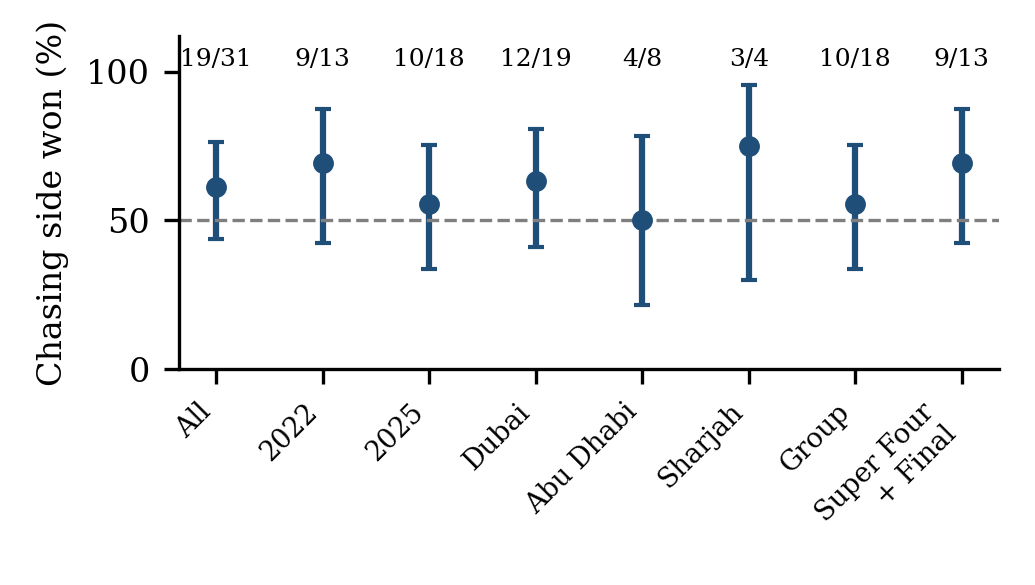
\includegraphics[width=\columnwidth]{fig1_chase_rate.png}
\caption{Share of matches won by the chasing side, with ranges. Labels show wins out of matches played. The dashed line is 50\%.}
\label{fig:chase}
\end{figure}

\runin{Does the toss help?} Toss winners won 19 of 32 matches (59.4\%, range 42 to 74\%, $p=0.38$), which is again not clearly different from chance. Captains liked to field first. They did so in 75\% of matches, in 85\% of matches in 2022 and in 68\% in 2025. Those who fielded won 15 of 24, and those who batted won 4 of 8.

\runin{How many runs are scored?} Sides batting first averaged 157.0 runs and sides batting second averaged 137.5 (Fig.~\ref{fig:scores}). A chase ends as soon as the target is reached, so many second innings stop early and the two averages should not be compared too closely. Powerplay runs are linked to the first innings total (Fig.~\ref{fig:pp}). The correlation is 0.44 with a range of 0.25 to 0.65, and each powerplay run goes with about 1.3 extra runs in the full innings.

\begin{figure}[!t]
\centering
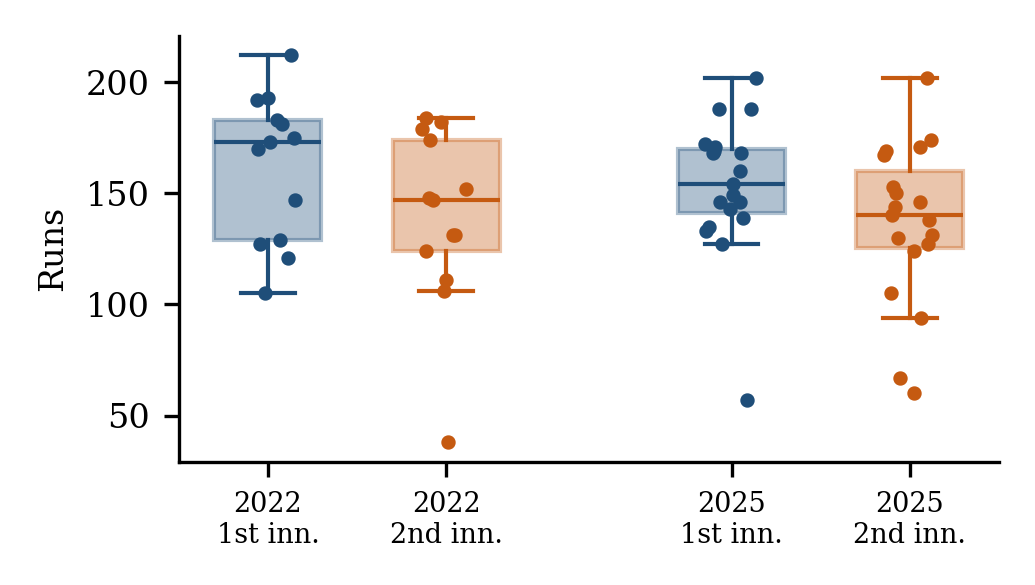
\includegraphics[width=\columnwidth]{fig2_innings_scores.png}
\caption{First and second innings totals in each tournament. Each dot is one match.}
\label{fig:scores}
\end{figure}

\begin{figure}[!t]
\centering
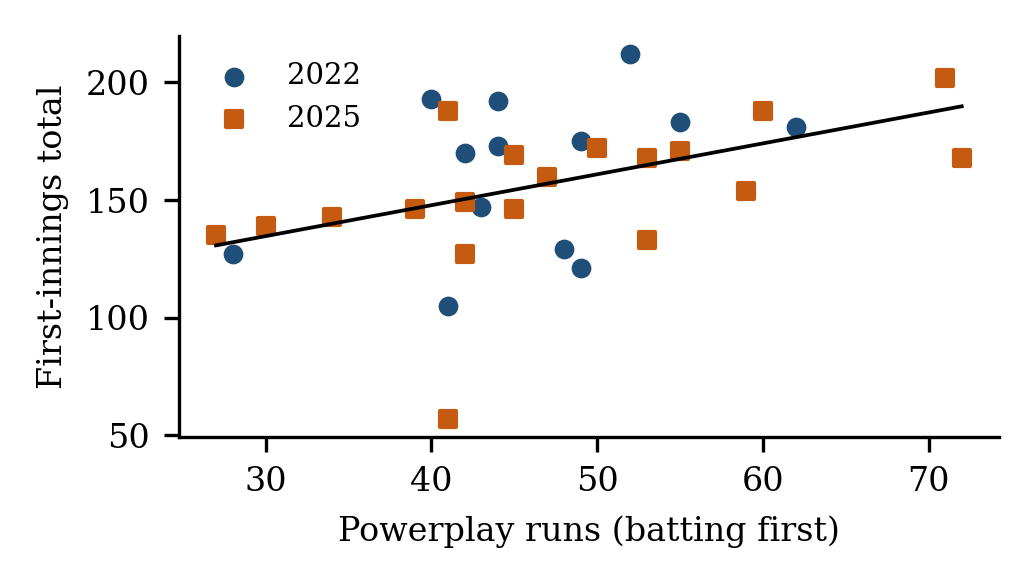
\includegraphics[width=\columnwidth]{fig3_powerplay.png}
\caption{First innings total against powerplay runs, with a straight line fit.}
\label{fig:pp}
\end{figure}

\runin{Allowing for team strength.} Some teams are simply stronger, so we gave every team an Elo rating \cite{elo1978}. The rating starts equal for the five full member teams, starts lower for Hong Kong, Oman and the UAE, and moves after every match. We then fitted a Bayesian model \cite{gelman2013} with a standard sampling method \cite{metropolis1953}. In plain terms, the model starts with a cautious guess and adjusts it as matches are added, and it returns a range instead of one number. For two equally strong teams, the chance that the chasing side wins is 0.67, with a range of 0.39 to 0.87, and a 91\% probability that it is above one half. The estimates for the grounds are Dubai 0.68, Abu Dhabi 0.63 and Sharjah 0.71. They overlap heavily (Fig.~\ref{fig:post}), so we cannot say that one ground favours chasing more than another. Team strength clearly matters, and stronger teams win more often.

\begin{figure}[!t]
\centering
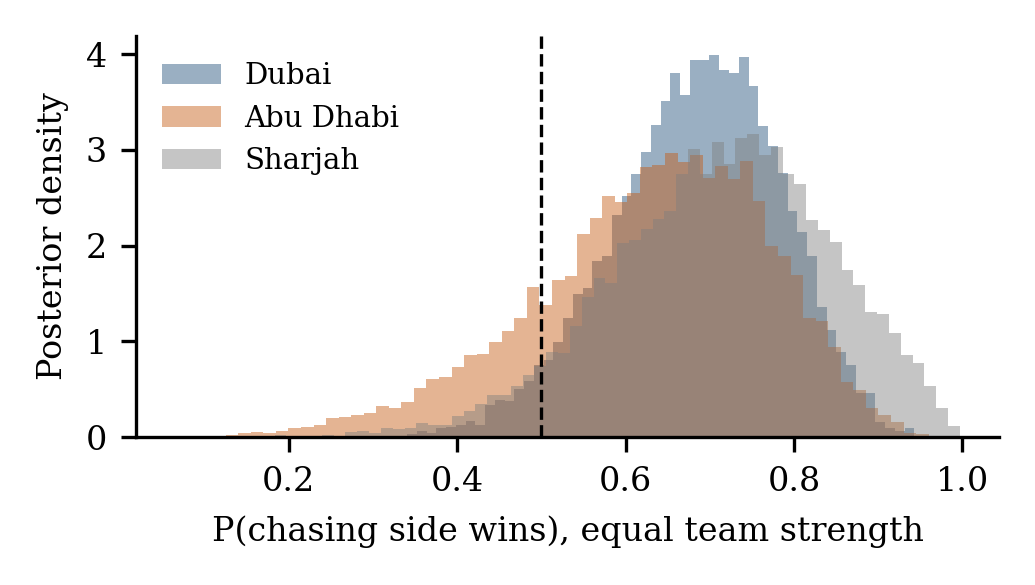
\includegraphics[width=\columnwidth]{fig4_posterior.png}
\caption{Likely values of the chance that the chasing side wins at each ground, for two equally strong teams. The dashed line is 50\%.}
\label{fig:post}
\end{figure}

\runin{Can a computer predict the winner?} We tried logistic regression, a random forest \cite{breiman2001} and gradient boosting \cite{friedman2002}. We compared them with two simple rules, which were to always pick the chasing side and to pick the higher rated team. We tested two moments. One was right after the toss, and the other was the break between innings, when the first score is known. To keep the test fair, every match was predicted by a model that had never seen it. Table~\ref{tab:models} and Fig.~\ref{fig:models} show the results. After the toss, logistic regression picked the winner in about 71\% of matches, against 61\% for always choosing the chasing side, and the Elo rule did about as well at 74\%. Adding the first score did not help much, and the best method at that moment was the random forest with 74\%. The ranges overlap, so no method is clearly better. We also shuffled the results 300 times to see how often luck alone could match our model. It did so about once in twenty tries ($p=0.053$), which is a hint and not proof. When we trained on one tournament and tested on the other, logistic regression reached 72\% (2022 to 2025) and 85\% (2025 to 2022). The random forest fell to 38\% in the second case, below the 56\% from always picking the chasing side. With data this small, a simple method is the safer choice.

\begin{table}[!t]
\caption{How often each method picked the winner (31 matches, each predicted without having been seen). Brier measures the error of the stated probabilities. Lower is better, and 0.25 is a coin flip.}
\label{tab:models}
\centering
\footnotesize
\renewcommand{\arraystretch}{1.05}
\begin{tabular}{@{}p{0.43\columnwidth}ccc@{}}
\toprule
\textbf{Method} & \textbf{Right (\%)} & \textbf{Range} & \textbf{Brier} \\
\midrule
\multicolumn{4}{@{}l}{\textit{Right after the toss}} \\
Always pick the chasing side & 61 & 45 to 77 & 0.24 \\
Logistic regression & 71 & 55 to 84 & 0.18 \\
Random forest & 71 & 55 to 84 & 0.19 \\
Gradient boosting & 68 & 52 to 84 & 0.21 \\
Pick the higher rated team & 74 & 58 to 87 & 0.20 \\
\midrule
\multicolumn{4}{@{}l}{\textit{At the break between innings}} \\
Logistic regression & 68 & 52 to 84 & 0.19 \\
Random forest & 74 & 58 to 87 & 0.20 \\
Gradient boosting & 71 & 55 to 87 & 0.24 \\
\bottomrule
\end{tabular}
\end{table}


\begin{figure}[!t]
\centering
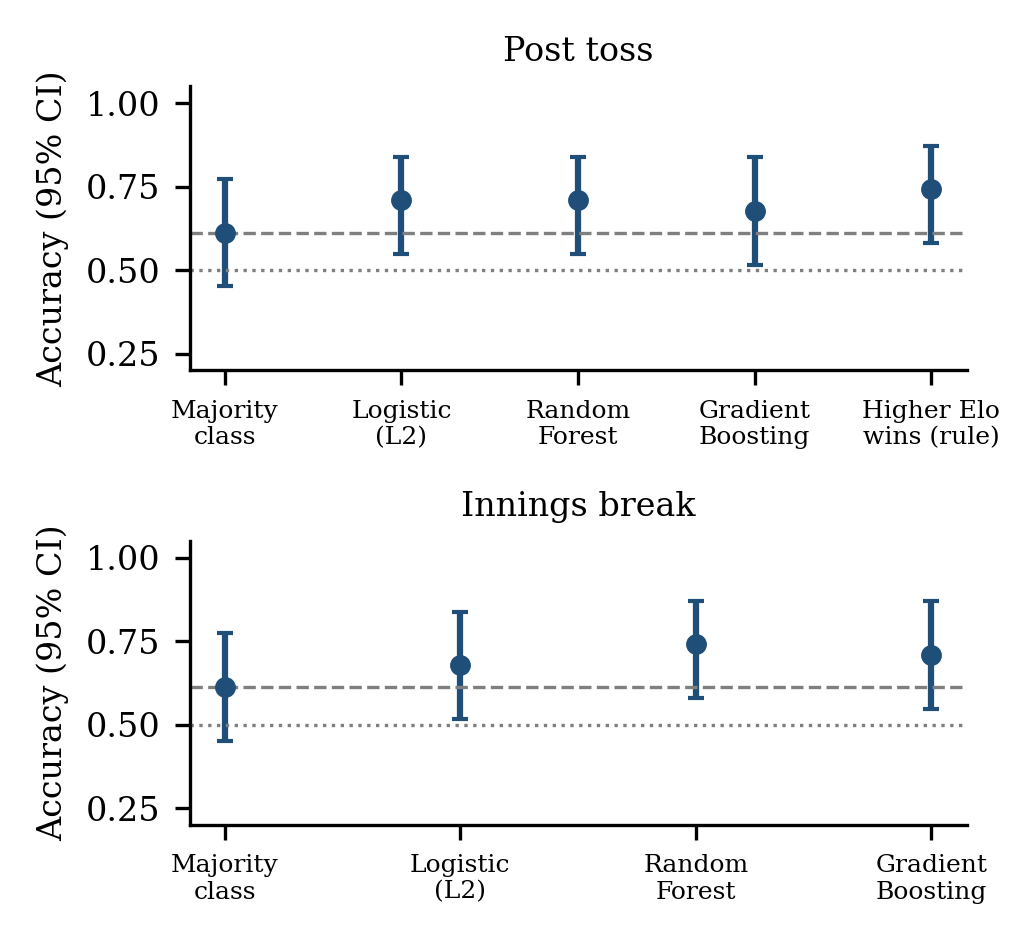
\includegraphics[width=\columnwidth]{fig5_models.png}
\caption{Share of matches predicted correctly, with ranges. The dashed line shows always picking the chasing side. The dotted line is 50\%.}
\label{fig:models}
\end{figure}

\section{Limitations and Usage Notes}
\label{sec:limits}
The dataset is small, with 32 matches from two tournaments. It suits exploring and teaching, but it cannot support strong claims about cricket in general. The 2025 temperature, humidity and wind figures are forecasts and not readings, and they are incomplete. The pitch notes record what previews and experts said. Abu Dhabi boundary lengths, wind direction and the 2025 reserve umpire are empty, and detailed scorecards exist for 2025 only. Sharjah appears only in 2022 and Abu Dhabi only in 2025, so the effect of a ground is hard to separate from the effect of a year. The team ratings use a lower starting value for Hong Kong, Oman and the UAE, which is our own judgement, and the results were not adjusted for the many questions asked.

The workbook opens in any spreadsheet program, and the master table can be read directly with tools such as Python and its \texttt{pandas} library. We suggest that users treat empty cells as missing and not as zero, keep the rule that Team~1 batted first, leave the Super Over match out of win and loss analysis, and read the source column before using a weather or pitch note. The 2025 base file is licensed under CC BY 4.0 \cite{razadata}, and we share AsiaCupT20 under the same licence. Please credit this paper and the original 2025 dataset when you use the data. Users should also check the terms of the original websites before reusing any text. The files and code are at \texttt{[repository link to be added]}, and the script reproduces every number and figure in Section~\ref{sec:analysis}.

\section{Conclusion}
We built a match level dataset of the 2022 and 2025 Asia Cup T20 tournaments. It holds 32 matches with 58 fields, a detailed sheet for 2025, and pitch and weather notes with their sources. We fixed errors in the source records, added calculated fields, and showed with automatic tests that the numbers agree. A first look suggests a mild lean towards chasing and little effect from the toss, but with so few matches both could be chance. We hope the dataset saves others the long job of collecting these records, and that it grows as more tournaments are added.

\section*{Acknowledgment}
The authors thank [names to be added] for their advice and support. We also thank Raza and Ali for releasing the 2025 dataset openly.


% Generated by IEEEtran.bst, version: 1.14 (2015/08/26)
\begin{thebibliography}{10}
\providecommand{\url}[1]{#1}
\csname url@samestyle\endcsname
\providecommand{\newblock}{\relax}
\providecommand{\bibinfo}[2]{#2}
\providecommand{\BIBentrySTDinterwordspacing}{\spaceskip=0pt\relax}
\providecommand{\BIBentryALTinterwordstretchfactor}{4}
\providecommand{\BIBentryALTinterwordspacing}{\spaceskip=\fontdimen2\font plus
\BIBentryALTinterwordstretchfactor\fontdimen3\font minus
  \fontdimen4\font\relax}
\providecommand{\BIBforeignlanguage}[2]{{%
\expandafter\ifx\csname l@#1\endcsname\relax
\typeout{** WARNING: IEEEtran.bst: No hyphenation pattern has been}%
\typeout{** loaded for the language `#1'. Using the pattern for}%
\typeout{** the default language instead.}%
\else
\language=\csname l@#1\endcsname
\fi
#2}}
\providecommand{\BIBdecl}{\relax}
\BIBdecl

\bibitem{razaarxiv}
K.~Raza and F.~Ali, ``Asia {C}up 2025: A structured {T}20 match-level dataset
  and exploratory analysis for cricket analytics,'' arXiv:2512.19740 [cs.LG],
  Dec. 2025.

\bibitem{razadata}
K.~Raza, ``Asia {C}up 2025 {T}20 match-level dataset,'' Zenodo, licence CC BY
  4.0, 2025.

\bibitem{bailey2006}
M.~Bailey and S.~R. Clarke, ``Predicting the match outcome in one day
  international cricket matches, while the game is in progress,'' \emph{Journal
  of Sports Science and Medicine}, vol.~5, no.~4, pp. 480--487, 2006.

\bibitem{asif2016}
M.~Asif and I.~G. McHale, ``In-play forecasting of win probability in one-day
  international cricket: A dynamic logistic regression model,''
  \emph{International Journal of Forecasting}, vol.~32, no.~1, pp. 34--43,
  2016.

\bibitem{morley2005}
B.~Morley and D.~Thomas, ``An investigation of home advantage and other factors
  affecting outcomes in {E}nglish one-day cricket matches,'' \emph{Journal of
  Sports Sciences}, vol.~23, no.~3, pp. 261--268, 2005.

\bibitem{kapadia2022}
K.~Kapadia, H.~Abdel-Jaber, F.~Thabtah, and W.~Hadi, ``Sport analytics for
  cricket game results using machine learning: An experimental study,''
  \emph{Applied Computing and Informatics}, vol.~18, no. 3/4, pp. 256--266,
  2022.

\bibitem{shah2025}
S.~A.~A. Shah, Q.~Zaman, D.~Wasim, J.~Allohibi, A.~A. Alharbi, and M.~Shabbir,
  ``Optimal model for predicting highest runs chase outcomes in {T}-20
  international cricket using modern classification algorithms,''
  \emph{Alexandria Engineering Journal}, vol. 114, pp. 588--598, Feb. 2025.

\bibitem{suseela2025}
G.~Suseela, B.~R. Devi, A.~Ashwitha, R.~Venkataramana, S.~J. Hussain, and
  J.~Avanija, ``Predictive analysis of cricket match outcomes: A comparative
  study of machine learning and data mining techniques,'' in \emph{Hybrid
  Intelligent Systems (HIS 2023)}, ser. Lecture Notes in Networks and Systems,
  A.~Bajaj, A.~M. Madureira, and A.~Abraham, Eds., vol. 1224.\hskip 1em plus
  0.5em minus 0.4em\relax Springer, 2025, pp. 425--432.

\bibitem{cricsheet}
{Cricsheet}, ``Cricsheet: Ball by ball data for cricket matches,''
  \url{https://cricsheet.org}, accessed: Oct. 25, 2026.

\bibitem{espn}
{ESPNcricinfo}, ``Asia {C}up 2025 match scorecards and reports,''
  \url{https://www.espncricinfo.com/series/men-s-t20-asia-cup-2025-1496919},
  accessed: Oct. 25, 2026.

\bibitem{acc}
{Asian Cricket Council}, ``Asia {C}up 2025 official tournament information,''
  \url{https://www.asiancricket.org}, accessed: Oct. 25, 2026.

\bibitem{wisden}
{Wisden}, ``Live cricket scores and match pages, {A}sia {C}up 2025,''
  \url{https://www.wisden.com/live-cricket-scores}, accessed: Oct. 25, 2026.

\bibitem{news}
{WION, Gulf News, Outlook India, CricTracker, and Cricket Times}, ``Asia {C}up
  2025 match previews, pitch reports and weather forecasts,'' Online articles
  at wionews.com, gulfnews.com, outlookindia.com, crictracker.com and
  crickettimes.com, accessed: Oct. 25, 2026.

\bibitem{wilson1927}
E.~B. Wilson, ``Probable inference, the law of succession, and statistical
  inference,'' \emph{Journal of the American Statistical Association}, vol.~22,
  no. 158, pp. 209--212, 1927.

\bibitem{pedregosa2011}
F.~Pedregosa \emph{et~al.}, ``Scikit-learn: Machine learning in {P}ython,''
  \emph{Journal of Machine Learning Research}, vol.~12, pp. 2825--2830, 2011.

\bibitem{elo1978}
A.~E. Elo, \emph{The Rating of Chessplayers, Past and Present}.\hskip 1em plus
  0.5em minus 0.4em\relax New York, NY, USA: Arco, 1978.

\bibitem{gelman2013}
A.~Gelman, J.~B. Carlin, H.~S. Stern, D.~B. Dunson, A.~Vehtari, and D.~B.
  Rubin, \emph{Bayesian Data Analysis}, 3rd~ed.\hskip 1em plus 0.5em minus
  0.4em\relax Boca Raton, FL, USA: CRC Press, 2013.

\bibitem{metropolis1953}
N.~Metropolis, A.~W. Rosenbluth, M.~N. Rosenbluth, A.~H. Teller, and E.~Teller,
  ``Equation of state calculations by fast computing machines,'' \emph{The
  Journal of Chemical Physics}, vol.~21, no.~6, pp. 1087--1092, 1953.

\bibitem{breiman2001}
L.~Breiman, ``Random forests,'' \emph{Machine Learning}, vol.~45, no.~1, pp.
  5--32, 2001.

\bibitem{friedman2002}
J.~H. Friedman, ``Stochastic gradient boosting,'' \emph{Computational
  Statistics \& Data Analysis}, vol.~38, no.~4, pp. 367--378, 2002.

\end{thebibliography}


\end{document}
